\documentclass{TDP003mall}
\usepackage{listings}
\usepackage{color}

\definecolor{keyword}{RGB}{168,27,166}
\definecolor{string}{RGB}{50,140,55}
\definecolor{number}{RGB}{153,105,0}
\definecolor{comment}{RGB}{160,161,167}


\lstset{frame=tb,
  language=Python,
  aboveskip=3mm,
  belowskip=3mm,
  showstringspaces=false,
  columns=flexible,
  basicstyle={\small\ttfamily},
  numbers=none,
  numberstyle=\tiny\color{number},
  keywordstyle=\color{keyword},
  commentstyle=\color{comment},
  stringstyle=\color{string},
  breaklines=true,
  breakatwhitespace=true,
  tabsize=3
}


\newcommand{\version}{Version 1.3}
\author{Anton Sköld, \href{mailto:antsk320@student.liu.se}{antsk320@student.liu.se}\\
  William Utbult, \href{mailto:wilut499@student.liu.se}{wilut499@student.liu.se}}
\title{TDP003 - Systemdokumentation}
\date{2017-10-10}
\rhead{Anton Sköld\\
William Utbult}



\begin{document}
\projectpage
\tableofcontents

\section{Revisionshistorik}
\begin{table}[!h]
\begin{tabularx}{\linewidth}{|l|X|c|}
\hline
Ver. & Revisionsbeskrivning & Datum \\\hline
1.0 & Grundläggande mall och Överblick tillagd & 2017-10-03\\\hline
1.1 & Lade till dokumentation för funktioner & 2017-10-09\\\hline
1.2 & Redigerad dokumentation över funktioner och tillagd sektion för tester, fel och loggning & 2017-10-10\\\hline
1.3 & Databasformat och språkversion tillagt & 2017-10-10\\\hline
\end{tabularx}
\end{table}


%Det skall finnas hänvisning till kursens specifikation av datalagret.
\section{Krav}
Se systemspecifikationsdokumenten:\\
\url{http://www.ida.liu.se/~TDP003/current/projekt/dokument/systemspecifikation.pdf} \\
\url{http://www.ida.liu.se/~TDP003/current/portfolio-api_python3/}


\section{Översikt}
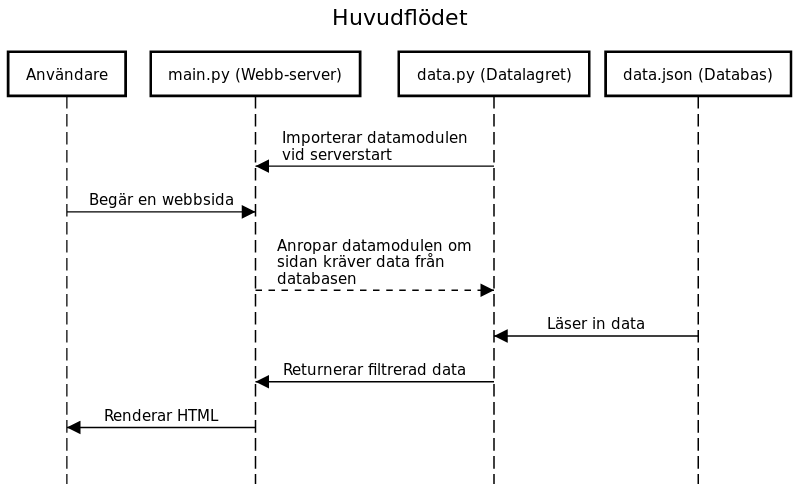
\includegraphics[width=17cm]{sequencediagram.org/mainflow2}
\hrule
1. Servern startar och importerar datamodulen

2. Användaren gör en http-begäran till servern

3. Om sidan kräver data från databasen anropas datamodulen

4. Databasen läses in

5. Datan filtreras och skickas tillbaka till servern

6. Servern renderar HTML med rätt inehåll och presenterar det för användaren

Steg 2-6 repeteras för varje http-begäran användaren gör.\\
Systemet är skrivet i Python 3.5.2 \& (Flask + Jinja2) för formatering och presentation i HTML5 \& CSS3.
Databasen i JSON-format ser ut som följande:
\begin{lstlisting}
[
  {
    "project_id": 1,

    "project_name": "Portfolio",

    "start_date": "2017-09-15",

    "end_date": "YYYY-MM-DD",

    "course_id": "TDP003",

    "course_name": "Projekt: Egna datormiljön",

    "techniques_used": ["HTML", "CSS", "Python"],

    "description": "Short description",

    "long_description": "Long description",

    "image": "https://url",

    "external_link": "https://url"
  },
  {...}
]
\end{lstlisting}


\section{Funktionförklaringar}
\subsection{main.py - Webbservern}
\subsubsection{\texttt{index()}}
Hämtar HTML för indexsidan och dess mallar\\
Anropas via Flask route "/"\\

\verb|   |\textbf{Returnerar: sträng}\\
\verb|   |\verb|   |HTML för indexsidan


\subsubsection{\texttt{search()}}
Läser in all input via HTML-form för sökningen
Hämtar sökresultaten från data.py och HTML för listsidan och dess mallar\\
Anropas via Flask route "/list/"\\

\verb|   |\textbf{Returnerar: sträng}\\
\verb|   |\verb|   |HTML för listsidan (med projekt matchande sökningen om sådan gjordes)


\subsubsection{\texttt{techniques()}}
Hämtar unika använda tekniker från data.py och HTML för techniquessidan och dess mallar\\
Anropas via Flask route "/techniques/"\\

\verb|   |\textbf{Returnerar: sträng}\\
\verb|   |\verb|   |HTML för techniquessidan (med alla unika använda tekniker i databasen)

\subsubsection{\texttt{project(id)}}
Hämtar projektinformation från data.py och HTML för projectsidan och dess mallar\\
Anropas via Flask route "/project/<id>" där id är projektets id\\

\verb|   |\textbf{Parametrar:}\\
\verb|   |\verb|   |id (heltal) - Projektets ID angivet i databasen

\verb|   |\textbf{Returnerar: sträng}\\
\verb|   |\verb|   |HTML för projectsidan (med projekt matchande sökningen om sådan gjordes)

\subsubsection{\texttt{page\_not\_found(e)}}
Hämtar HTML för 404sidan och dess mallar\\
Anropas via Flask errorhandler(404)\\
e har felkod och felmeddelande\\

\verb|   |\textbf{Parametrar:}\\
\verb|   |\verb|   |e (sträng) - Felkod och felmeddelande (ges av Flask)

\verb|   |\textbf{Returnerar: sträng}\\
\verb|   |\verb|   |HTML för 404sidan (e används inte för tillfället)


\subsection{data.py - Datalagret}
\subsubsection{\texttt{load(filename)}}
Läser in JSON-formaterad projektdata från den givna filen och returnerar en lista av projekt sorterade efter ID.\\

  \verb|   |\textbf{Parametrar:}\\
  \verb|   |\verb|   |filename (sträng) - filnamn/sökväg

  \verb|   |\textbf{Returnerar: lista}\\
  \verb|   |\verb|   |Lista innehållande en tabell per projekt (se databasen)

\subsubsection{\texttt{get\_project\_count(db)}}
Returnerar antalet projekt i en projektlista.\\
db är den givna listan.

  \verb|   |\textbf{Parametrar:}\\
  \verb|   |\verb|   |db (lista) - databas/projektlista

  \verb|   |\textbf{Returnerar: heltal}\\
  \verb|   |\verb|   |Antalet proejekt i databasen/listan

\subsubsection{\texttt{get\_project(db, id)}}
Returnerar ett projekt med givet id från projektlista.\\
db är den givna listan.\\
id är ID fär projektet som ska returneras.\\

\verb|   |\textbf{Parametrar:}\\
\verb|   |\verb|   |db (lista) - databas/projektlista\\
\verb|   |\verb|   |id (heltal) - projekt ID

\verb|   |\textbf{Returnerar: tabell}\\
\verb|   |\verb|   |Projektet inehållande projektinformation

\subsubsection{\texttt{search(db, sort\_by, sort\_order, techniques, search, search\_fields}}
Hittar och returnerar projekt från projektlista som matchar givna kriterier.\\

\verb|   |\textbf{Parametrar:}\\
\verb|   |\verb|   |\verb|db| (lista) - databas/projektlista\\
\verb|   |\verb|   |\verb|sort_by| (sträng) - fält som resultaten sorteras efter (se databas). Standard: "\verb|start_date|"\\
\verb|   |\verb|   |\verb|sort_order| (sträng) - Sorteringsordning. 'asc' för stigande, 'desc' för fallande. Standard: 'desc'\\
\verb|   |\verb|   |\verb|techniques| (lista) - List över använda tekniker (strängar) där alla måste matcha med projektet\\
\verb|   |\verb|   |\verb|search| (sträng) - sökord att matcha med projektinformation\\
\verb|   |\verb|   |\verb|search_field| (lista) - Lista över fält (strängar) att matcha sökord med (se databas).\\\verb|   |\verb|   |\verb|   |None ger alla. Standard: None\\

\verb|   |\textbf{Returnerar: tabell}\\
\verb|   |\verb|   |Projektet inehållande projektinformation


\subsubsection{\texttt{get\_techniques(db)}}
Returnerar en lista av alla unika använda tekniker i den givna databasen\\

\verb|   |\textbf{Parametrar:}\\
\verb|   |\verb|   |\verb|db| (lista) - databas/projektlista\\

\verb|   |\textbf{Returnerar: lista}\\
\verb|   |\verb|   |Tekniker (strängar)

\subsubsection{\texttt{get\_technique\_stats(db)}}
Samlar statistik över alla tekniker i den specificerade projektlistan.\\
Returnerar en tabell med alla unika använda tekniker och listor över vilka projekt som använde dem\\

\verb|   |\textbf{Parametrar:}\\
\verb|   |\verb|   |\verb|db| (lista) - databas/projektlista\\

\verb|   |\textbf{Returnerar: tabell}\\
\verb|   |\verb|   |Tabell av tekniker (listor) som i sin tur innehåller tabeller med 'id' = projektid, 'name' = projektnamn

\section{Tester, felhantering och loggning}
\subsection{Tester}
\subsubsection{Datalagret}
Datalagret fungerar just nu precis som det ska. Om ändringar skulle ske i det så finns det flera sätt att testa så att funktionerna fortfarande beter sig som de ska.\\\\
Första sättet är att kolla i källkoden, längst ner i data.py så finns det en hel del utkommenterade tester som vi skapade under utveckling av datalagret. De testar olika funktioner, och många kombinationer av sökparametrar. Man måste manuellt jämföra returdatat ur testerna med data.json-filen för att få reda på om det är det förväntade datat som returneras.\\\\
Andra sättet är genom de gemensamma testfallen som skapades dels av klassen och dels av kursledare.\\
De gemensamma testerna finns tillgängliga i \url{https://gitlab.ida.liu.se/filst04/tdp003-2017-database-tests/tree/master}.\\
För att använda de gemensamma testerna så klonar du repositoryt till lokal maskin, sedan kopiera in \verb|data.py| (Namn är viktigt) i mappen, och sedan kör \verb|data_test.py| med valfri modern Python-interpretator.\\
Sedan skrivs det ut information i terminalen om hur många tester som godkändes/misslyckades och hänvisar till vilka tester det var.

\subsubsection{Presentationslagret}
Presentationslagret har inte några specifika tester så som datalagret har. Omfattningen av möjliga tester skulle vara att göra sina ändringar, ladda om webbsidan, och läsa eventuella felmeddelanden.

\subsection{Felhantering}
\subsubsection{Datalagret}
Fel som uppstår inom datalagret är aldrig dödliga. De fel som kan uppstå, som att en fil inte finns eller att man har matat in dålig information, returnerar antingen tomma listor, eller ett None-objekt. När det sker så får man dubbelkolla sin input, och sedan stegvis gå igenom källkoden för att hitta de logiska buggarna.

\subsubsection{Presentationslagret}
Det fel som hanteras i presentationslagret just nu är 404-fel, att sidorna inte kan hittas.\\
Om man vill hantera ännu fler fel och man vet felkoden för felen så finns en @app.errorhandler(felkod) funktion tillgänglig i Flask. Den kan användas före en funktion för att få felhantering för det felet inuti funktionen.\\
De fel som kan uppstå under utveckling när man har dålig data/ofullständig kod med mera är oftast Jinja2-fel. Jinja2 har en inbyggd debugger som visar de senaste funktionsanropen som skedde innan felet uppstod.

\subsection{Loggning}
Datalagret och presentationslagret saknar loggning.\\
OpenShift (som systemet ligger på) har inbyggd loggning över vissa fel och händelser.\\
För att se webbserverns senaste log, kör kommandot \verb|"rhc tail portfolio"|, detta rekommenderas att vara körande vid uppdatering av sidan.\\

\end{document}
